\documentclass[tikz, margin=2]{standalone}
\usepackage{amsmath}


\begin{document}
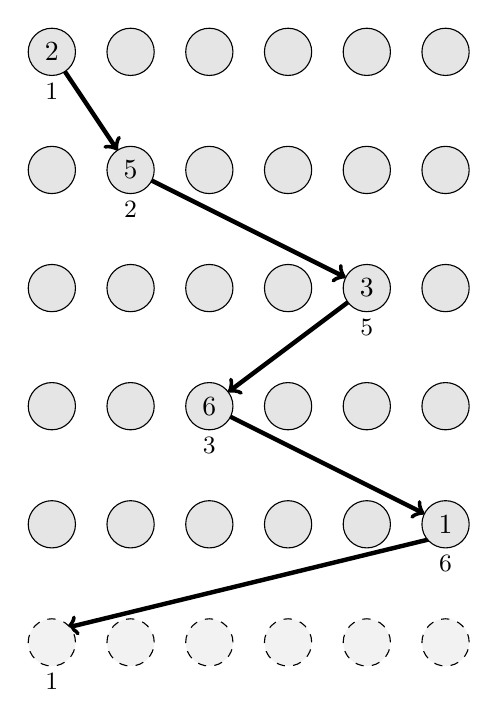
\begin{tikzpicture}

% Draw the arrows for the path
\draw[ultra thick,->] (.166,-.250) -- (.834,-1.250);
\draw[ultra thick,->] (1.268,-1.634) -- (3.732,-2.866);
\draw[ultra thick,->] (3.76,-3.18) -- (2.24,-4.32);
\draw[ultra thick,->] (2.268,-4.634) -- (4.732,-5.866);
\draw[ultra thick,->] (4.813,-6.186) -- (.187,-7.314);

% Draw all the columns in all the rows
\foreach \x in {0,1,...,5} {
    % Draw all the rows except the last
    \foreach \y in {0,-1.5,...,-6} {
        \filldraw[draw=black,fill=lightgray!40] (\x,\y) circle (.3);
    }
    % Draw the last row
    \filldraw[draw=black,dashed,fill=lightgray!20] (\x,-7.5) circle (.3);
}

% Draw the node indices and pointers
\foreach[
    evaluate=\i as \nx using {{0,1,4,2,5,0}[\i]},
    evaluate=\i as \ny using -1.5*\i),
    evaluate=\nx as \nn using {{1,2,3,4,5,6}[\nx]},
    evaluate=\i as \np using {{2,5,3,6,1,}[\i]},
] \i in {0,1,2,3,4,5} {
    \node at (\nx,\ny-.5) {\small{\nn}};
    \node at (\nx,\ny) {\np};
}

\end{tikzpicture}
\end{document}
